\documentclass[9pt,mathserif]{beamer}
%\documentclass[9pt,mathserif,handout]{beamer}
\mode<presentation>
{
  \usetheme{Warsaw}
  \usecolortheme{crane}
  \setbeamercovered{transparent}
	\useoutertheme{split} 
	 
	\defbeamertemplate*{slidenumber}{framenumber} 
	     {\insertframenumber} 
	 \defbeamertemplate{slidenumber}{totalframenumber} 
	     {\insertframenumber\,/\,\inserttotalframenumber} 
	 \defbeamertemplate{slidenumber}{pagenumber} 
	     {\insertpagenumber} 
	 \defbeamertemplate{slidenumber}{totalpagenumber} 
	     {\insertpagenumber\,/\,\insertpresentationendpage} 
	 
	\defbeamertemplate*{footline}{split slidenumber right} 
	 {% 
	   \leavevmode% 
	   \hbox{\begin{beamercolorbox}
	[wd=.5\paperwidth,ht=2.5ex,dp=1.125ex,leftskip=.3cm plus1fill,rightskip=.3cm]
	{author in head/foot}% 
	     \usebeamerfont{author in head/foot}\insertshortauthor 
	   \end{beamercolorbox}% 
	   \begin{beamercolorbox}
	[wd=.5\paperwidth,ht=2.5ex,dp=1.125ex,leftskip=.3cm,rightskip=.3cm plus1fil]
	{title in head/foot}% 
	     \usebeamerfont{title in head/foot}\insertshorttitle% 
	     \hskip2ex plus1fill% 
	     \usebeamertemplate{slidenumber}% 
	   \end{beamercolorbox}}% 
	   \vskip0pt% 
	 
	} 
	 
	\defbeamertemplate{footline}{split slidenumber left} 
	 {% 
	   \leavevmode% 
	   \hbox{\begin{beamercolorbox}
	[wd=.5\paperwidth,ht=2.5ex,dp=1.125ex,leftskip=.3cm plus1fil,rightskip=.3cm]
	{author in head/foot}% 
	     \usebeamerfont{author in head/foot}% 
	     \usebeamertemplate{slidenumber}% 
	     \hskip2ex plus1fill% 
	     \insertshortauthor 
	   \end{beamercolorbox}% 
	   \begin{beamercolorbox}
	[wd=.5\paperwidth,ht=2.5ex,dp=1.125ex,leftskip=.3cm,rightskip=.3cm plus1fil]
	{title in head/foot}% 
	     \usebeamerfont{title in head/foot}\insertshorttitle% 
	   \end{beamercolorbox}}% 
	   \vskip0pt% 
	} 
}

\usepackage[english]{babel}
\usepackage[latin1]{inputenc}
\usepackage{times}
\usepackage[T1]{fontenc}
\usepackage{verbatim}

\usepackage{amsmath}
\usepackage{amssymb}
\usepackage{amsfonts}
\usepackage{pxfonts}
\usepackage{amsthm}
\usepackage{graphicx}
\usepackage{stmaryrd}


\usepackage{bussproofs}
\usepackage{proof}

\usepackage{fancybox}
\usepackage{fancyvrb}

% \usepackage{tikz}
% \usepackage{pgfgantt}
% \usepackage{chronology}


%\usepackage{rotating}

% Sequent Calculus Proof Settings
\EnableBpAbbreviations
\def\fCenter{\mbox{\ $\vdash$\ }}

\usepackage{calculi}

% Logical symbols
\newcommand{\imp}{\rightarrow}
\newcommand{\biimp}{\leftrightarrow}
\newcommand{\all}{\forall}
\newcommand{\ex}{\exists}
\newcommand{\seq}{\vdash}
\newcommand{\nec}{\Box} % necessarily
\newcommand{\pos}{\Diamond} % possibly


\newcommand{\ess}[2]{#1 \ \mathit{ess} \ #2}
\newcommand{\NE}{E}

\newcommand{\s}{\qquad}

\def\modal#1{\boldsymbol{#1}}
\def\mfalse{\modal\bot}
\def\mtrue{\modal\top}
\def\mnot{\modal\neg\,}
\def\mor{\,\modal\vee\,}
\def\mand{\,\modal\wedge\,}
\def\mimpl{\,\modal\supset\,}
\def\miff{\,\modal\Leftrightarrow\,}
\def\mball#1{\modal\Box_{#1}\,}
\def\mdexi#1{\modal\Diamond_{#1}\,}
\def\mall#1{\modal{\forall}{#1}\lambdot\,}
\def\mallprop#1{\modal{\forall^{p}}{#1}\lambdot\,}
\def\mallind#1{\modal{\forall^{\mu}}{#1}\lambdot\,}
\def\mexi#1{\modal{\exists}{#1}\lambdot\,}
\def\mpi{\modal{\Pi}\,}
\def\mvalid{\modal{\texttt{valid}}} 

\def\typearrow{\shortrightarrow}
\def\worldtype{\iota}
\def\indtype{\mu}


\newenvironment{transitionframe}
{
\begin{frame}{} \Large
\centering
\colorbox{black}{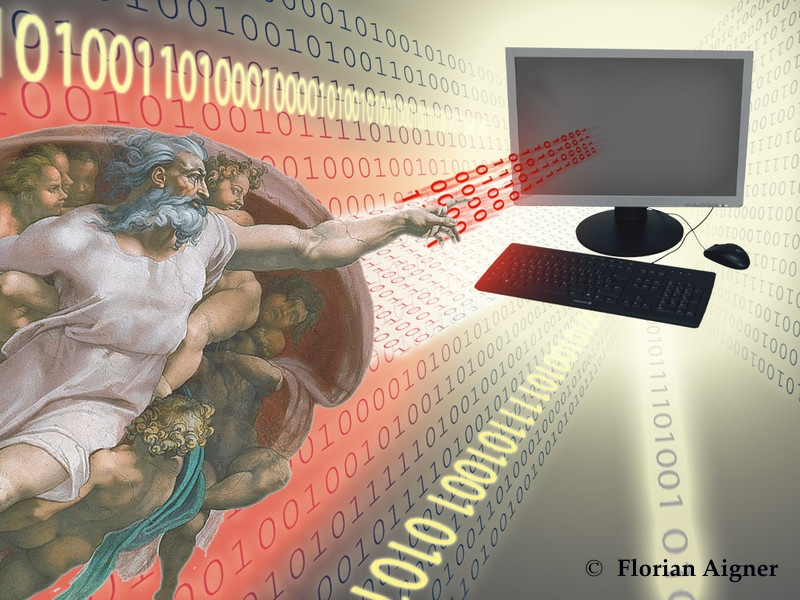
\includegraphics[width=.7\textwidth]{TUWien-GodComputerC}} 
\vfill
}
{

\end{frame}
}

\newenvironment{changemargin}[2]{% 
  \begin{list}{}{% 
    \setlength{\topsep}{0pt}% 
    \setlength{\leftmargin}{#1}% 
    \setlength{\rightmargin}{#2}% 
    \setlength{\listparindent}{\parindent}% 
    \setlength{\itemindent}{\parindent}% 
    \setlength{\parsep}{\parskip}% 
  }% 
\item[]
}{\end{list}} 


\title[On G\"{o}del's Proof of God's
Existence]{Formalization, Mechanization and Automation of \\ G\"{o}del's
  Proof of God's Existence}

\author{\textbf{Christoph Benzm\"{u}ller} and \textbf{Bruno Woltzenlogel Paleo}}

% \institute[]{
%   \inst{}%
% }

\date[1.11.2013]{November 1, 2013}

\begin{document}

\begin{frame}
  \titlepage
\colorbox{gray}{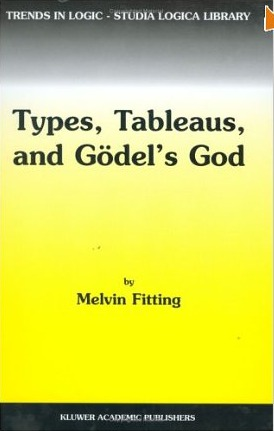
\includegraphics[height=2.5cm]{buch7.jpg} }
\hfill
\colorbox{gray}{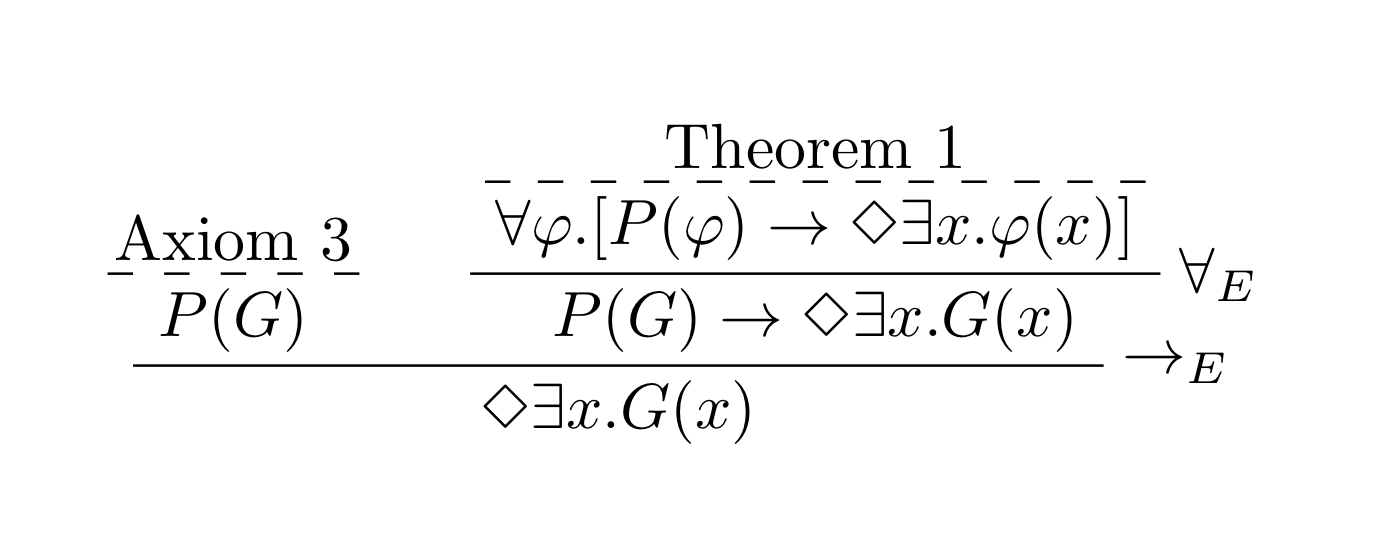
\includegraphics[height=2.5cm]{nd.png}}

\hfill \begin{footnotesize}A gift to \textbf{Priest Edvaldo} and his church in Piracicaba, Brazil\end{footnotesize}
\end{frame}


\begin{frame}{} \small
\vskip1em
\begin{minipage}{.56\textwidth} 
\colorbox{gray}{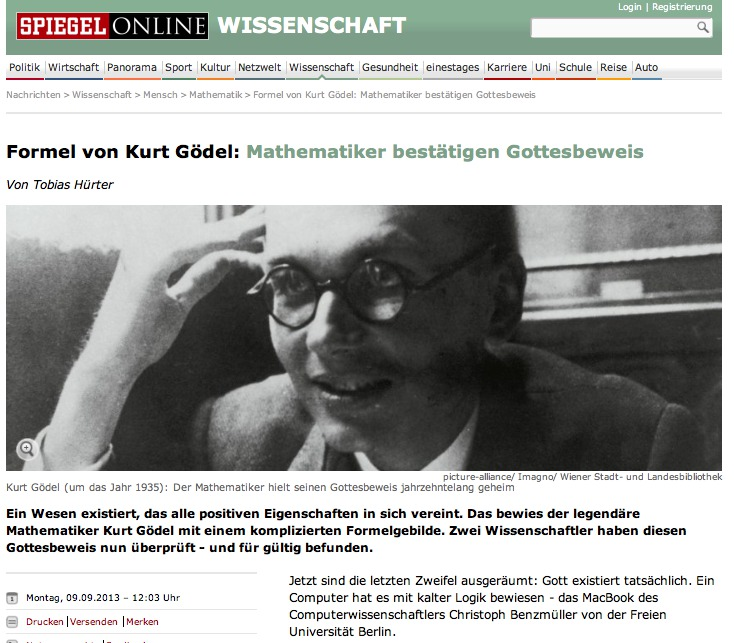
\includegraphics[width=\textwidth]{spiegel1}} 
\vskip1em
Germany \\
- Telepolis \& Heise \\
- Spiegel Online \\
- FAZ \\
- Die Welt \\
- Berliner Morgenpost \\
- Hamburger Abendpost \\
- \ldots \\
\end{minipage} \hfill
%
\begin{minipage}{.3\textwidth}
Austria \\
- Die Presse \\
- Wiener Zeitung \\
- ORF \\
- \ldots \\

Italy \\
- Repubblica \\
- Ilsussidario \\
- \ldots \\

% Russia \\
% - \ldots \\

India \\
- DNA India \\
- Delhi Daily News \\
- India Today \\
- \ldots \\

US \\
- ABC News \\
- \ldots \\

International \\
- Spiegel International \\
- Yahoo Finance \\
% - CNET \\
- United Press Intl. \\
- \ldots \\
\end{minipage}
\end{frame}

\begin{frame}{Introduction --- Quick answers to your most pressing questions!} \large
\colorbox{gray}{
\includegraphics[width=\textwidth]{MacBookGrab}} 
\pause
\vfill
Are we in contact with Steve Jobs? \hfill No \\[2em]
Do you really need a MacBook to obtain the results? \hfill No \\[2em]
Is Apple sending us money? \hfill No \\
\, \hfill (but maybe they should)
\end{frame}

\begin{frame}{Introduction}\large
%Ontological argument: Conclude that God exists from premises by pure, a priori reasoning.
\begin{block}{Def: \textcolor{blue}{Ontological Argument/Proof}}
* deductive argument \\

* for the existence of god \\

* starting from premises, which are justified by pure reasoning,
i.e. they do not depend on observation in the world.
\end{block}

\vfill \pause
Existence of God: different types of arguments/proofs\\[.2em]
\begin{itemize}
\item[---]a posteriori (use experience/observation in the world)
  \begin{itemize}
  \item[------]teleological
  \item[------]cosmological
  \item[------]moral
  \item[------] \ldots
  \end{itemize}  
\item[---]a priori (based on pure reasoning, independent)
  \begin{itemize}
  \item[------]\textcolor{blue}{ontological argument}
    \begin{itemize}
    \item[------]definitional 
    \item[------]modal 
    \item[------] \ldots
    \end{itemize}
  \item[------]other a priori arguments
  \end{itemize}
\end{itemize}
\end{frame}

\begin{frame}{Introduction}

\emph{\huge Wohl eine jede Philosophie kreist um den ontologischen
  Gottesbeweis} \\[2em]
(Adorno, Th. W.: Negative Dialektik. Frankfurt a. M. 1966, p.378)
\vfill
\ldots \hfill
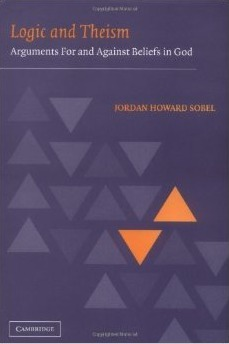
\includegraphics[height=2cm]{buch3.jpg} \hfill
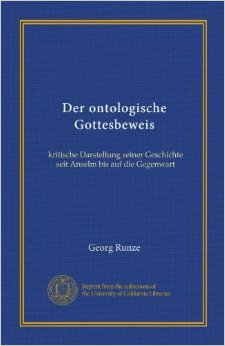
\includegraphics[height=2cm]{buch2.jpg} \hfill 
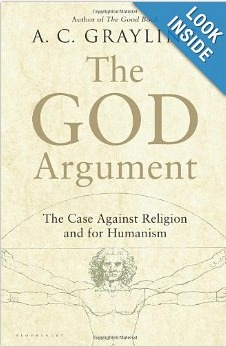
\includegraphics[height=2cm]{buch4.jpg} \hfill
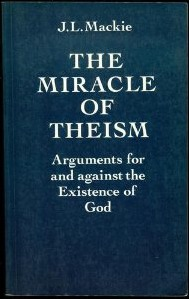
\includegraphics[height=2cm]{buch5.jpg} \hfill
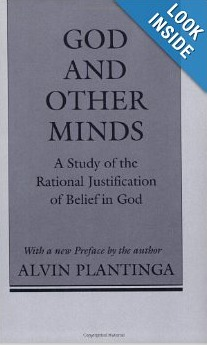
\includegraphics[height=2cm]{buch6.jpg} \hfill

\includegraphics[height=2cm]{buch1.jpg} \hfill
\ldots
\end{frame}


\begin{frame}{Introduction} \Large
{Rich history on ontological arguments (\textcolor{blue}{pros} and \textcolor{red}{cons})}\\[1em]

\hskip-.5em
\ldots\rotatebox[origin = bl,width = 0mm]{65}{\textcolor{blue}{Anselm v. C.}} \hskip-2.3em
\ldots  \rotatebox[origin = bl]{65}{\textcolor{red}{Th. Aquinas}}  \hskip-2.3em
\ldots\ldots   \rotatebox[origin = bl]{65}{\textcolor{blue}{Descartes}} \hskip-1.7em
               \rotatebox[origin = bl]{65}{\textcolor{blue}{Spinoza}} \hskip-1.3em
               \rotatebox[origin = bl]{65}{\textcolor{blue}{Leibniz}}  \hskip-1.2em
\ldots  \rotatebox[origin = bl]{65}{\textcolor{red}{Hume}}  \hskip-1em
          \rotatebox[origin = bl]{65}{\textcolor{red}{Kant}}  \hskip-.8em
\ldots  \rotatebox[origin = bl]{65}{\textcolor{blue}{Hegel}}  \hskip-1.3em
\ldots  \rotatebox[origin = bl]{65}{\textcolor{red}{Frege}}  \hskip-1.3em
\ldots  \rotatebox[origin = bl]{65}{\textcolor{blue}{Hartshorne}} \hskip-1.9em
          \rotatebox[origin = bl]{65}{\textcolor{blue}{Malcolm}}  \hskip-1.4em
          \rotatebox[origin = bl]{65}{\textcolor{red}{Lewis}}  \hskip-1em
          \rotatebox[origin = bl]{65}{\textcolor{blue}{Plantinga}}  \hskip-1.6em
          \rotatebox[origin = bl]{65}{\textcolor{blue}{G\"odel}}   \hskip-1.2em
\ldots \\[1em]

\pause
\vfill
Anselm's notion of God:\\
\,\hfill \emph{``God is that, than which nothing greater can be
  conceived.''} \\[1em]

G\"odel's notion of God:\\
\,\hfill \emph{``A God-like being possesses all `positive' properties.''} \\[1em]

To show by logical reasoning: \\
\,\hfill \emph{``(Necessarily) God exists.''} \\[1em]

% \rnode{n2}{}\emph{}
% \ncline[nodesep=2pt,linecolor=black,linewidth=1pt]{->}{n1}{n2}
\end{frame}


\begin{frame}{Introduction} \Large
Different Interests in Ontological Arguments: \\[1em]
\begin{itemize}
\item \textcolor{blue}{Philosophical:} Boundaries of Metaphysics \& Epistemology
  \begin{itemize}
  \item We talk about a metaphysical concept (God), 
  \item but we want to draw
      a conclusion for the real world. \\[1em]
  \item Necessary Existence (NE): metaphysical NE vs. logical NE  vs. modal NE \\[2em]
  \end{itemize} 
\item \textcolor{blue}{Theistic:} Successful argument should convince atheists. \\[2em]
\item \textcolor{red}{Our:} Can computers (theorem provers) be used
  \begin{itemize}
  \item to formalize the definitions and axioms?
  \item to verify the arguments step-by-step?
  \item to fully automate (sub-)arguments? \\[1em]
  \end{itemize}
  \textcolor{red}{\emph{``Computer-assisted Theoretical Philosophy''}}
\end{itemize}
\end{frame}

\begin{frame}{Introduction} \large
Main challenge: \hfill No provers for \emph{Higher-order Modal Logic\/} (\textcolor{red}{HML}) \\[1em]

Our solution: \hfill Embedding in \emph{Higher-order Classical Logic\/} (\textcolor{blue}{HOL}) \\
\,\hfill {\small [Benzm\"ullerPaulson, Logica Universalis, 2013]} \\[2em]

What we did \textcolor{blue}{(rough outline for remaining
  presentation!)}: \\

\begin{itemize}
\item[A:] pen and paper: detailed natural deduction proof 
\item[B:] formalization: in classical higher-order logic (\textcolor{blue}{HOL})
\item[] proof automation: theorem provers \textsc{Leo-II} and \textsc{Satallax} 
\item[] consistency: model finder \textsc{Nitpick (Nitrox)} 
\item[C:] step-by-step verification: proof assistant \textsc{Coq} 
\item[D:] automation \& verification: proof assistant 
  \textsc{Isabelle} \\[2em]
%\item[ ] Conclusion \\[2em]
\end{itemize}
Did we get new results? \hfill  \textcolor{red}{Yes --- let's discuss later!}
\end{frame}


\begin{transitionframe}{Images/Transitions/RioChrist3}
\textbf{Part A:}

Informal Proof and Natural Deduction Proof
\end{transitionframe}




\begin{frame}{G\"odel's Manuscript (1970)}
\bigskip

\begin{changemargin}{-1.2cm}{-1.2cm}
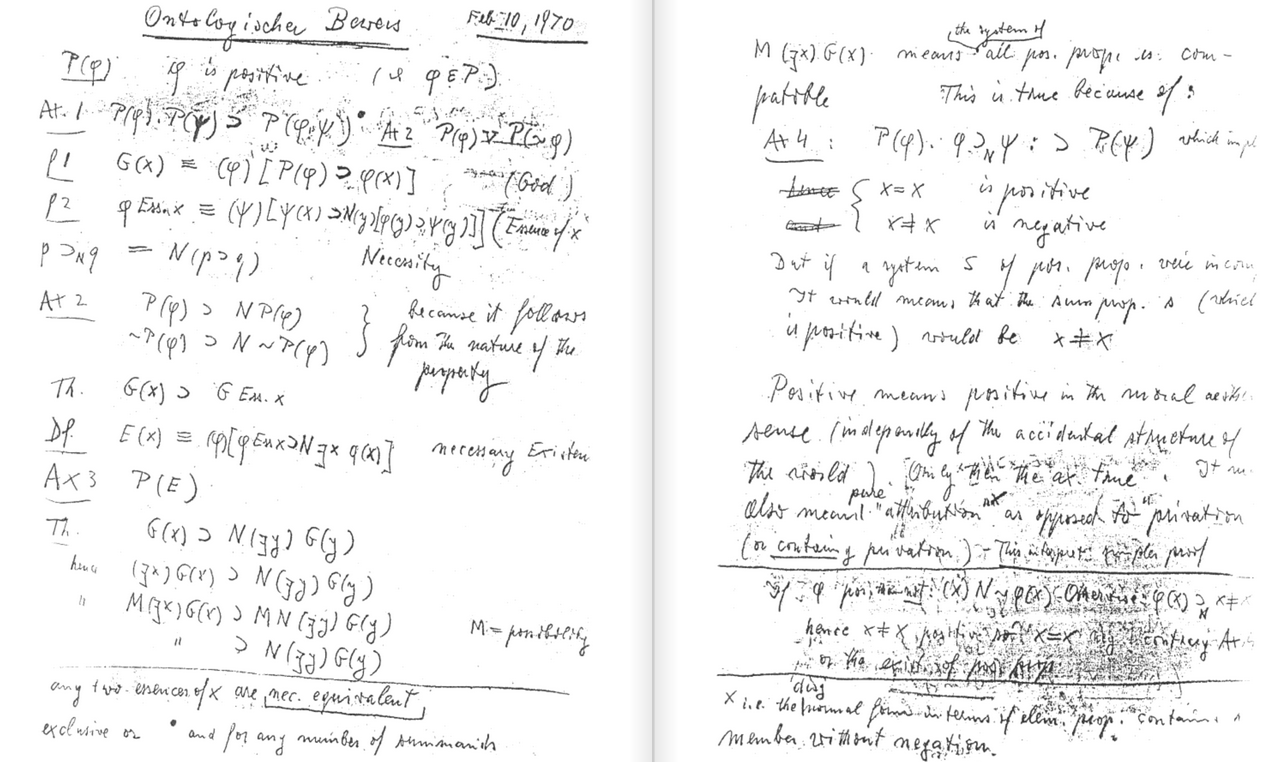
\includegraphics[width=13cm]{Images/Manuscript.png}
\end{changemargin}
\end{frame}

\begin{frame}{Scott's Version of G\"odel's Axioms, Definitions and Theorems}
\begin{changemargin}{-0.9cm}{-0.8cm}
\colorbox{black}{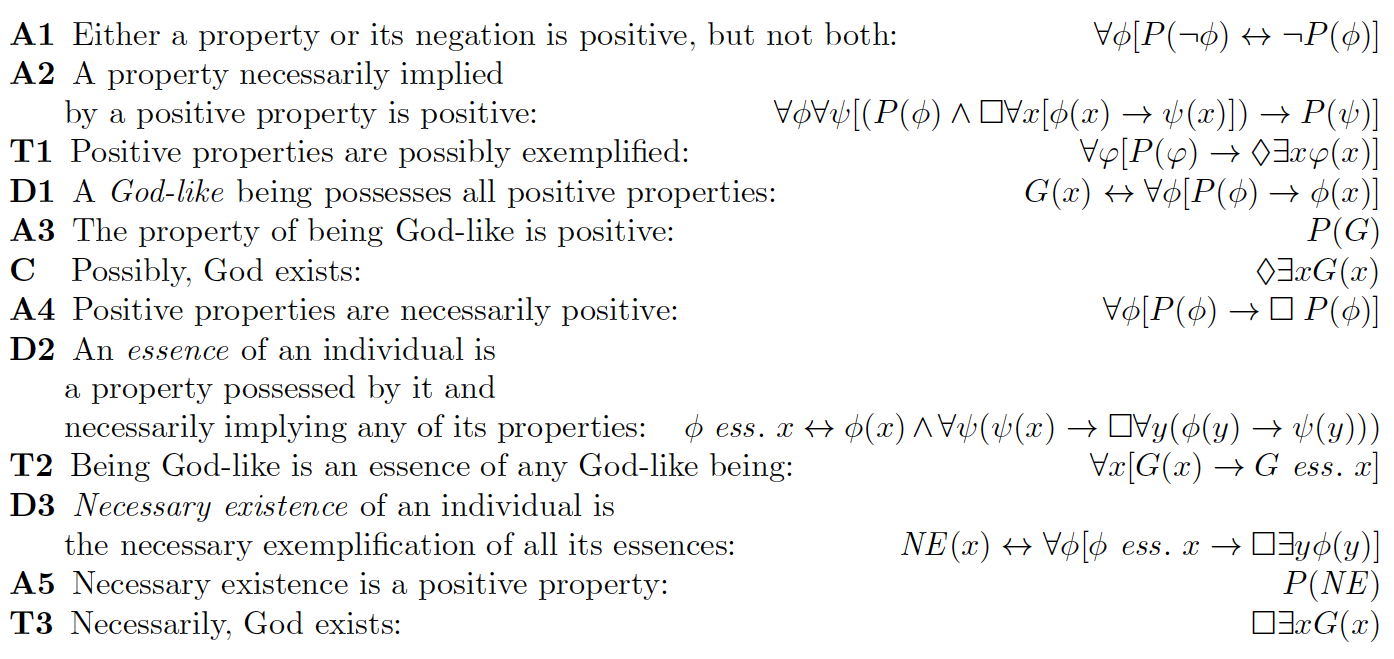
\includegraphics[width=12.4cm]{Images/ScottsScriptGrab.png}}
\end{changemargin}
\end{frame}


\begin{frame}[shrink]{Proof Overview}

$$
\textbf{D1: } G(x) \equiv \forall \varphi. [P(\varphi) \to \varphi(x)]
$$

$$
\textbf{D2: } \ess{\varphi}{x} \equiv \varphi(x) \wedge \all \psi. (\psi(x) \imp \nec \all x. (\varphi(x) \imp \psi(x)))
$$

$$
\textbf{D3: } E(x) \equiv \all \varphi.[\ess{\varphi}{x} \imp \nec \ex y.\varphi(y)]
$$

\begin{prooftree}
\AXC{$\textbf{A3}$} \dashedLine
\UIC{$P(G)$}
		\AXC{$\textbf{A2}$} \dashedLine
		\UIC{$\all \varphi. \all \psi.[(P(\varphi) \wedge \nec \all x.[\varphi(x) \imp \psi(x)]) \imp P(\psi)]$}
					\AXC{$\textbf{A1a}$} \dashedLine
					\UIC{$\all \varphi. [P(\neg \varphi) \imp \neg P(\varphi)]$} \doubleLine
				\BIC{$\textbf{T1: } \all \varphi. [P(\varphi) \imp \pos \ex x.\varphi(x)]$} \doubleLine
	\BIC{$\textbf{C1: } \pos \ex x. G(x)$}
\end{prooftree}



\begin{prooftree}
						\AXC{$\textbf{A1b}$} \dashedLine
						\UIC{$\all \varphi. [\neg P(\varphi) \imp P(\neg \varphi)]$}
								\AXC{$\textbf{A4}$} \dashedLine
								\UIC{$ \all \varphi.[P(\varphi) \to \Box \; P(\varphi)] $} \doubleLine
							\BIC{$\textbf{T2: } \all y.[G(y) \imp \ess{G}{y}]$}
									\AXC{$\textbf{A5}$} \dashedLine
									\UIC{$ P(E) $} \doubleLine
								\BIC{$\textbf{L1: } \ex z. G(z) \imp \nec \ex x. G(x)$} \doubleLine
								\UIC{$\pos \ex z. G(z) \imp \pos \nec \ex x. G(x)$}
										\AXC{$\textbf{S5}$} \dashedLine
 										\UIC{$ \all \xi.[\pos \nec \xi \imp \nec \xi]$} \doubleLine	
									\BIC{$\textbf{L2: } \pos \ex z. G(z) \imp \nec \ex x. G(x)$}
\end{prooftree}

\begin{prooftree}
\AXC{$\textbf{C1: } \pos \ex x. G(x)$}
		\AXC{$\textbf{L2: } \pos \ex z. G(z) \imp \nec \ex x. G(x)$} \doubleLine
	\BIC{$\textbf{T3: } \nec \ex x. G(x) $}
\end{prooftree}

\end{frame}

\begin{frame}[shrink]{Natural Deduction Calculus}

\begin{unnamedCalculus}

\vspace{1em}

\s\s
\infer[\vee_E]{C}{A \vee B & \infer*{C}{\infer{A}{}} & \infer*{C}{\infer{B}{}}}
\s\s
\infer[\wedge_I]{A \wedge B}{A & B}
\s\s
\infer[\imp_I^n]{A \imp B}{ \infer*{B}{\infer[n]{A}{}} }

\vspace{2em}

\s\s
\infer[\vee_{I_1}]{A \vee B}{A}
\s\s
\infer[\wedge_{E_1}]{A}{A \wedge B}
\s\s
\infer[\imp_I]{A \imp B}{ B }

\vspace{2em}

\s\s
\infer[\vee_{I_2}]{A \vee B}{B}
\s\s
\infer[\wedge_{E_2}]{B}{A \wedge B}
\s\s
\infer[\imp_E]{B}{A & A \imp B}

\vspace{2em}

\s
\infer[\all_I]{\all x. A[x]}{ A[\alpha] }
\s
\infer[\all_E]{A[t]}{ \all x. A[x] }
\s\s
\infer[\ex_I]{\ex x. A[x]}{ A[t] }
\s
\infer[\ex_E]{A[\beta]}{ \ex x. A[x] }

\vspace{1em}

\s\s\s\s
$\neg A \equiv A \imp \bot$ 
\s\s\s 
\alert{\infer[\neg\neg_E]{A}{\neg\neg A}}

\vspace{1em}

\end{unnamedCalculus}

\end{frame}



\begin{frame}[shrink]{Natural Deduction Calculus}{Rules for Modalities}

\begin{unnamedCalculus}

\vspace{1em}

\s\s\s\s
\infer[\nec_I]{\nec A}{\alpha: \fbox{\infer*{A}{}} }
\s\s\s\s\s
\infer[\nec_E]{t: \fbox{ \infer*{}{A} }  }{\nec A}

\vspace{2em}

\s\s\s\s
\infer[\pos_I]{\pos A}{t: \fbox{\infer*{A}{}} }
\s\s\s\s\s
\infer[\pos_E]{\beta: \fbox{ \infer*{}{A} }  }{\pos A}

\vspace{2em}

\alert{$$\pos A \equiv \neg \nec \neg A$$}

\vspace{1em}

\end{unnamedCalculus}

\end{frame}



\begin{frame}{Natural Deduction Proofs}{T1 and C1}
\begin{prooftree}
        \AXC{\textbf{A2}} \dashedLine
        \UIC{$ \all \varphi. \all \psi.[(P(\varphi) \wedge \nec \all x.[\varphi(x) \imp \psi(x)]) \imp P(\psi)]$} \RightLabel{$\all_E$}
        \UIC{$ \all \psi.[(P(\rho) \wedge \nec \all x.[\rho(x) \imp \psi(x)]) \imp P(\psi)]$} \RightLabel{$\all_E$}
        \UIC{$(P(\rho) \wedge \nec \all x.[\rho(x) \imp \neg \rho(x)]) \imp P(\neg \rho)$} \doubleLine
        \UIC{$(P(\rho) \wedge \nec \all x.[\neg \rho(x)]) \imp P(\neg \rho)$}
                        \AXC{\textbf{A1a}} \dashedLine
                        \UIC{$\all \varphi.[ P(\neg \varphi) \imp \neg P(\varphi) ]$} \RightLabel{$\all_E$}
                        \UIC{$ P(\neg \rho) \imp \neg P(\rho) $} \doubleLine
                 \BIC{$ (P(\rho) \wedge \nec \all x.[\neg \rho(x)]) \imp \neg P(\rho) $} \doubleLine
                 \UIC{$ P(\rho) \imp \pos \ex x.\rho(x) $} \RightLabel{$\all_I$}
                 \UIC{$\all \varphi.[ P(\varphi) \imp \pos \ex x.\varphi(x) ] $}
\end{prooftree}

\begin{prooftree}
\AXC{\textbf{A3}} \dashedLine
\UIC{$P(G)$}
                 \AXC{\textbf{T1}} \dashedLine
                 \UIC{$\all \varphi.[ P(\varphi) \imp \pos \ex x.\varphi(x) ]$} \RightLabel{$\all_E $}
                 \UIC{$ P(G) \imp \pos \ex x.G(x) $} \RightLabel{$\imp_E$}
    \BIC{$\pos \ex x. G(x)$}
\end{prooftree}
\end{frame}



\begin{frame}{Natural Deduction Proofs}{T2 (Partial)}
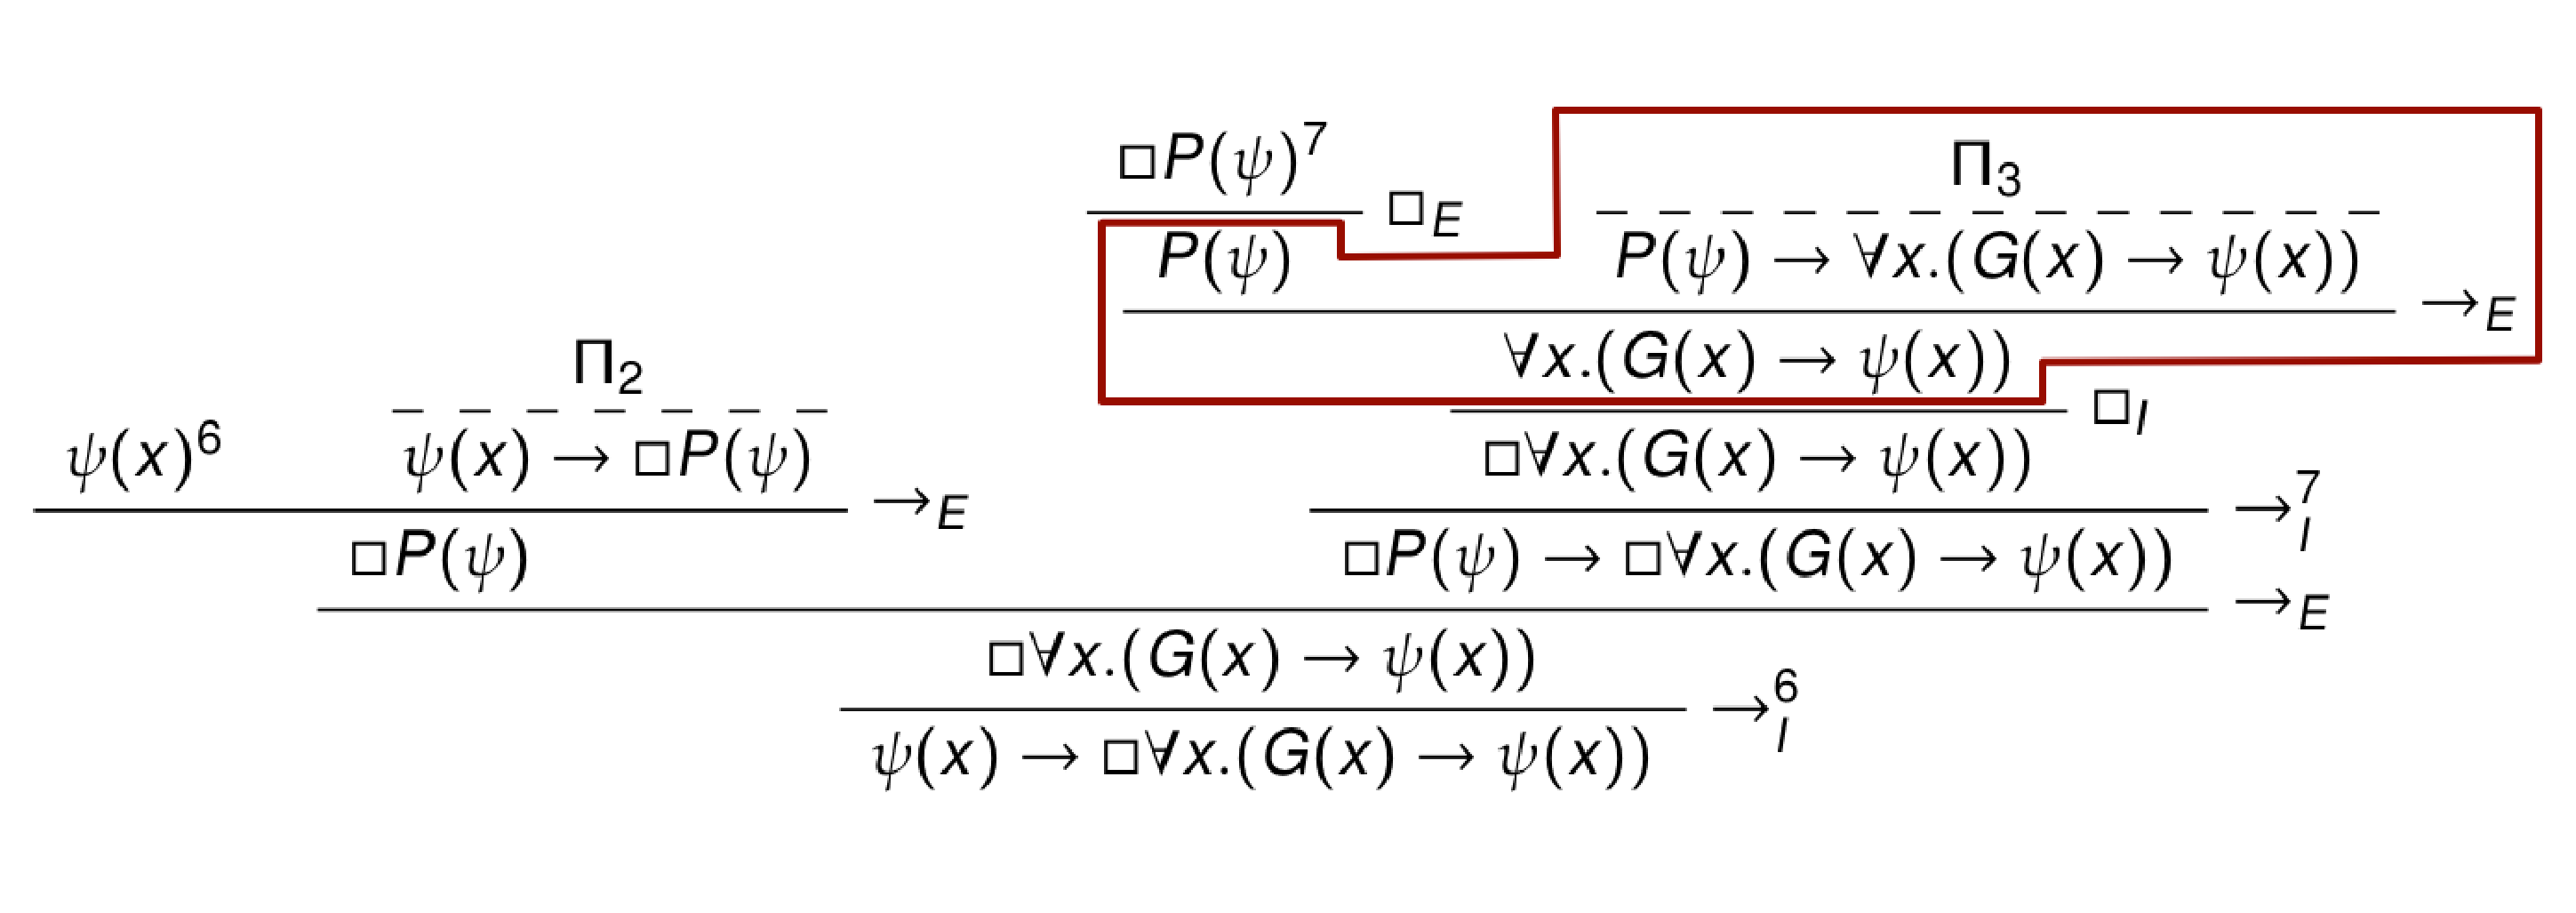
\includegraphics[scale=0.22]{Images/ProofOfT2Boxed.pdf}
\end{frame}


\begin{transitionframe}{}
\textbf{Part B:} \\[.5em]
\quad Formalization: \hfill in classical higher-order logic (\textcolor{black}{HOL}) \\
\quad Automation: \hfill theorem provers \textsc{Leo-II} and \textsc{Satallax} \\ 
\quad Consistency: \hfill model finder \textsc{Nitpick (Nitrox)} \\
\end{transitionframe}

\begin{frame}{Formalization in HOL} \large

\hskip-1em Challenge: \hfill No provers for \emph{Higher-order
  Quantified Modal
  Logic\/} (\textcolor{red}{QML}) \\[1em]

\hskip-1em Our solution: \hfill Embedding in \emph{Higher-order Classical
  Logic\/} (\textcolor{blue}{HOL}) \\
\, \hfill Then use existing \textcolor{blue}{HOL} theorem provers for reasoning in \textcolor{red}{QML} \\
\,\hfill {\small [Benzm\"ullerPaulson, Logica Universalis, 2013]}
\\[2em]

Previous empiricial findings:  \\[.5em]
\,\hfill Embedding of  \emph{First-order Modal Logic} in HOL works well 

\,\hfill {\small [Benzm\"ullerOttenRaths, ECAI, 2012]} \\
\,\hfill {\small [Benzm\"uller, LPAR, 2013]}
\end{frame}



\begin{frame}{Formalization in HOL} \large

\hskip-1em\textcolor{red}{QML} \hfill
$\begin{array}{lll}\textcolor{red}{\varphi,\psi} & ::= &
  \textcolor{red}{\ldots}  \mid \textcolor{red}{\neg
    \varphi} \mid \textcolor{red}{\varphi \wedge \psi} \mid
  \textcolor{red}{\varphi \imp \psi}  \mid \textcolor{red}{\Box
    \varphi} \mid \textcolor{red}{\Diamond \varphi}  \mid
  \textcolor{red}{\forall {x}\, \varphi} \mid
  \textcolor{red}{\exists {x}\, \varphi} 
\mid \textcolor{red}{\forall {P}\, \varphi} \end{array}$ \\[1em]


\begin{itemize}
\item Kripke style semantics (possible world semantics)\\[2em]
\end{itemize}



\hskip-1em\textcolor{blue}{HOL}\hfill 
$\begin{array}{lll}
\textcolor{blue}{s,t} & ::= & \textcolor{blue}{C}  \mid
\textcolor{blue}{x \mid \lambda{x} s} \mid \textcolor{blue}{s\, t}
\mid \textcolor{blue}{\neg s} \mid \textcolor{blue}{s \vee t} \mid
\textcolor{blue}{\forall {x}\, t} 
\end{array}$ \\[1em]

\begin{itemize}
\item meanwhile very well understood
\item Henkin semantics vs. standard semantics
\item various theorem provers do exists \\[.5em]
  \quad interactive: \hfill Isabelle/HOL, HOL4, Hol Light, Coq/HOL, PVS,
  \ldots \\[.5em]
  \quad automated: \hfill TPS, LEO-II, Satallax, Nitpick, Isabelle/HOL, \ldots \\
\end{itemize}


\end{frame}


\begin{frame}{Formalization in HOL}\large

\hskip-1em\textcolor{red}{QML} \hfill
$\begin{array}{lll}\textcolor{red}{\varphi,\psi} & ::= &
  \textcolor{red}{\ldots}  \mid \textcolor{red}{\neg
    \varphi} \mid \textcolor{red}{\varphi \wedge \psi} \mid
  \textcolor{red}{\varphi \imp \psi}  \mid \textcolor{red}{\Box
    \varphi} \mid \textcolor{red}{\Diamond \varphi}  \mid
  \textcolor{red}{\forall {x}\, \varphi} \mid
  \textcolor{red}{\exists {x}\, \varphi} 
\mid \textcolor{red}{\forall {P}\, \varphi} \end{array}$ \\[1.5em]

\hskip-1em\textcolor{blue}{HOL}\hfill 
$\begin{array}{lll}
\textcolor{blue}{s,t} & ::= & \textcolor{blue}{C}  \mid
\textcolor{blue}{x \mid \lambda{x} s} \mid \textcolor{blue}{s\, t}
\mid \textcolor{blue}{\neg s} \mid \textcolor{blue}{s \vee t} \mid
\textcolor{blue}{\forall {x}\, t} 
\end{array}$ \\[1.5em]


\hskip-1em\textcolor{red}{QML} in \textcolor{blue}{HOL}: \quad \textcolor{red}{QML}
formulas $\textcolor{red}{\varphi}$ are mapped to
\textcolor{blue}{HOL} predicates $\textcolor{red}{\varphi_{\worldtype\typearrow o}}$

\begin{center}
\fcolorbox{blue}{white}{
$\begin{array}{lcl} 
    \textcolor{red}{\mnot} & = & \textcolor{blue}{
      \lambda{\varphi_{\worldtype\typearrow o}}\lambda{s_\worldtype}\neg \varphi s} \\ 
    \textcolor{red}{\mand} & = & \textcolor{blue}{ 
      \lambda{\varphi_{\worldtype\typearrow o}}
      \lambda{\psi_{\worldtype\typearrow o}} \lambda{s_\worldtype}
      (\varphi s \wedge \psi s)} \\ 
    \textcolor{red}{\imp} & = & \textcolor{blue}{ 
      \lambda{\varphi_{\worldtype\typearrow o}}
      \lambda{\psi_{\worldtype\typearrow o}} \lambda{s_\worldtype}
      (\neg \varphi s \vee \psi s)} \\ 
    \textcolor{red}{\Box} & = & \textcolor{blue}{ 
      \lambda{\varphi_{\worldtype\typearrow o}} \lambda{s_\worldtype}
      \forall {u_\worldtype}\, (\neg r s u \vee
      \varphi u)} \\ 
    \textcolor{red}{\Diamond} & = & \textcolor{blue}{ 
      \lambda{\varphi_{\worldtype\typearrow o}} \lambda{s_\worldtype}
      \exists {u_\worldtype}\, (r s u \wedge
      \varphi u)} \\ 
    \textcolor{red}{\forall} & = & \textcolor{blue}{ 
      \lambda{h_{\mu\typearrow(\worldtype \typearrow o)}}
      \lambda{s_\worldtype} \forall {d_\indtype} \, h d s} \\
    \textcolor{red}{\exists} & = & \textcolor{blue}{ 
      \lambda{h_{\mu\typearrow(\worldtype \typearrow o)}}
      \lambda{s_\worldtype} \exists {d_\indtype} \, h d s} \\
    \textcolor{red}{\forall} & = & \textcolor{blue}{ 
      \lambda{H_{(\mu\typearrow(\worldtype \typearrow o))\typearrow(\worldtype \typearrow o)}}
      \lambda{s_\worldtype} \forall {d_\indtype} \, H d s} \\
    \\
      \text{\textcolor{brown}{valid}} & = & \textcolor{blue}{
        \lambda{\varphi_{\worldtype\typearrow o}} \all{w_\worldtype}
        \varphi w}
\end{array}$
}  \quad \textcolor{blue}{Ax} 
\vskip1em
\end{center}
\quad The equations in \textcolor{blue}{Ax} are given as axioms to the \textcolor{blue}{HOL} provers! \\
\quad \textcolor{gray}{\small (Remark: We are here dealing with constant domain quantification.)}

\end{frame}



\begin{frame}{Formalization in HOL} \large

\hskip-1em Example \\[.5em]

 \textcolor{red}{QML} formula  \hfill \textcolor{red}{$\Diamond \exists x G(x)$}

 \textcolor{red}{QML} formula in \textcolor{blue}{HOL}  \hfill $\text{\textcolor{brown}{valid}}\, \textcolor{red}{(\Diamond \exists x G(x))_{\worldtype\typearrow o}}$

expansion, $\beta\eta$-conversion \hfill $\textcolor{blue}{\forall
  w_\worldtype\textcolor{red}{(\Diamond \exists x
    G(x))_{\worldtype\typearrow o}}\, w}$ 

expansion, $\beta\eta$-conversion \hfill $\textcolor{blue}{\forall
  w_\worldtype \exists {u_\worldtype} (r w u \wedge
      \textcolor{red}{(\exists x G(x))_{\worldtype\typearrow o}} u)}$ 

% expansion, $\beta\eta$-conversion \hfill $\textcolor{blue}{\forall
%   w_\worldtype \exists {u_\worldtype} (r w u \wedge
%       \exists x \textcolor{red}{G(x)_{\worldtype\typearrow o}} u)}$ 

expansion, $\beta\eta$-conversion \hfill $\textcolor{blue}{\forall
  w_\worldtype \exists {u_\worldtype} (r w u \wedge
      \exists x G x u)}$ \\[1em]
\pause
\vfill
\begin{block}{What are we doing?}
\vskip.5em
In order to prove that $\textcolor{red}{\varphi}$ is valid in \textcolor{red}{QML}, \\
--> we instead prove that 
$\text{\textcolor{brown}{valid}}\,
\textcolor{red}{\varphi_{\worldtype\typearrow o}}$ can be derived
from \textcolor{blue}{Ax} in \textcolor{blue}{HOL}. \\[1em]

This can be done with interactive or automated \textcolor{blue}{HOL} theorem provers.
\end{block}
\pause
\vfill
\hskip-1em Expansion: \hfill user or prover may flexibly choose expansion depth \\[.5em]

\end{frame}


\begin{frame}{Automated Theorem Provers and Model Finders for HOL}
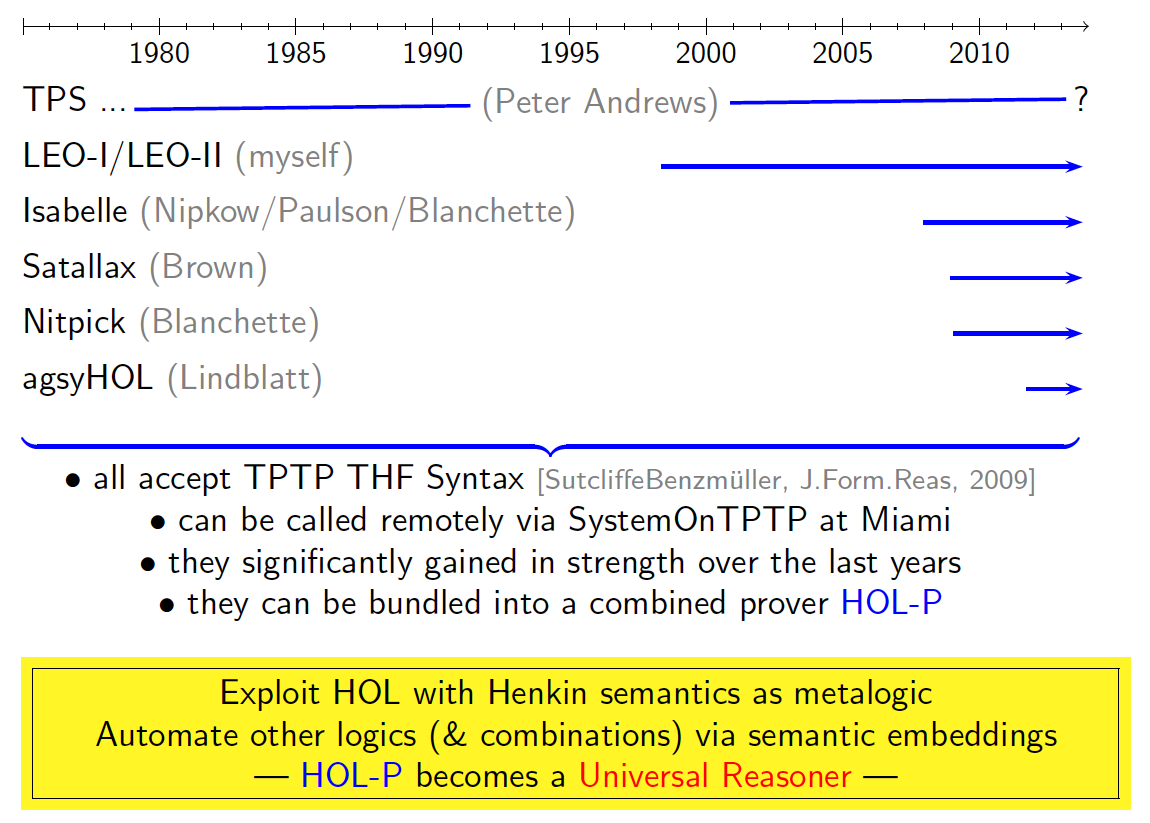
\includegraphics[width=1.05\textwidth]{HOLProversGrab}
\end{frame}


\begin{frame}{Proof Automation and Consistency Checking: Demo!} \large
\colorbox{gray}{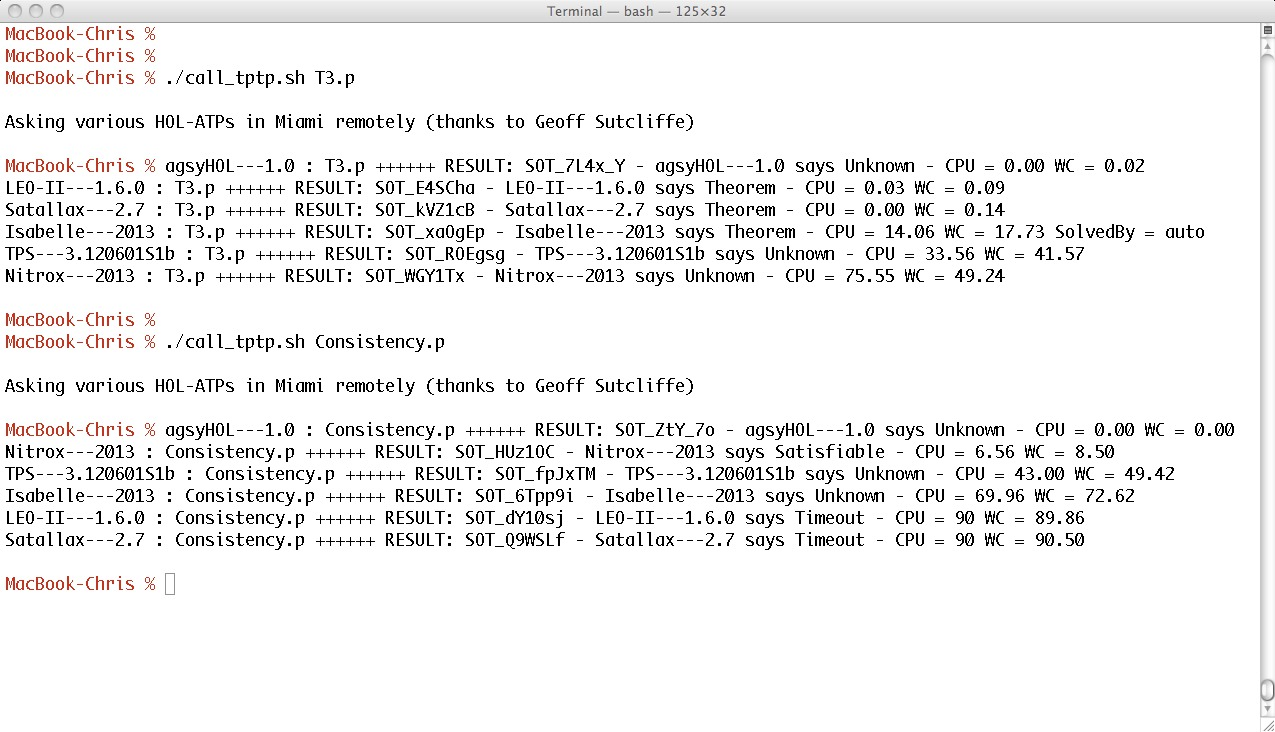
\includegraphics[width=\textwidth]{DemoGrap}} 
\vfill 
Provers are called remotely in Miami --- no local installation needed!
\end{frame}



\begin{frame}{Coq Proof}{Demo} \small
\begin{itemize}
\item Goal: verification of the natural deduction proof
\begin{itemize}
\item Step-by-step formalization
\item Almost no automation (intentionally!)
\end{itemize}
%
\item Interesting facts to note:
\begin{itemize}
\item Embedding is transparent to the user
\item Embedding gives labeled calculus for free
\end{itemize}
\end{itemize}
\end{frame}



\begin{transitionframe}{} \Large \centering
\textbf{Part D:} \\[.5em]
\quad automation \& verification: proof assistant \textsc{Isabelle} \\[2em]
\end{transitionframe}

\begin{frame}{} \Large \centering
\vskip.5em
\colorbox{gray}{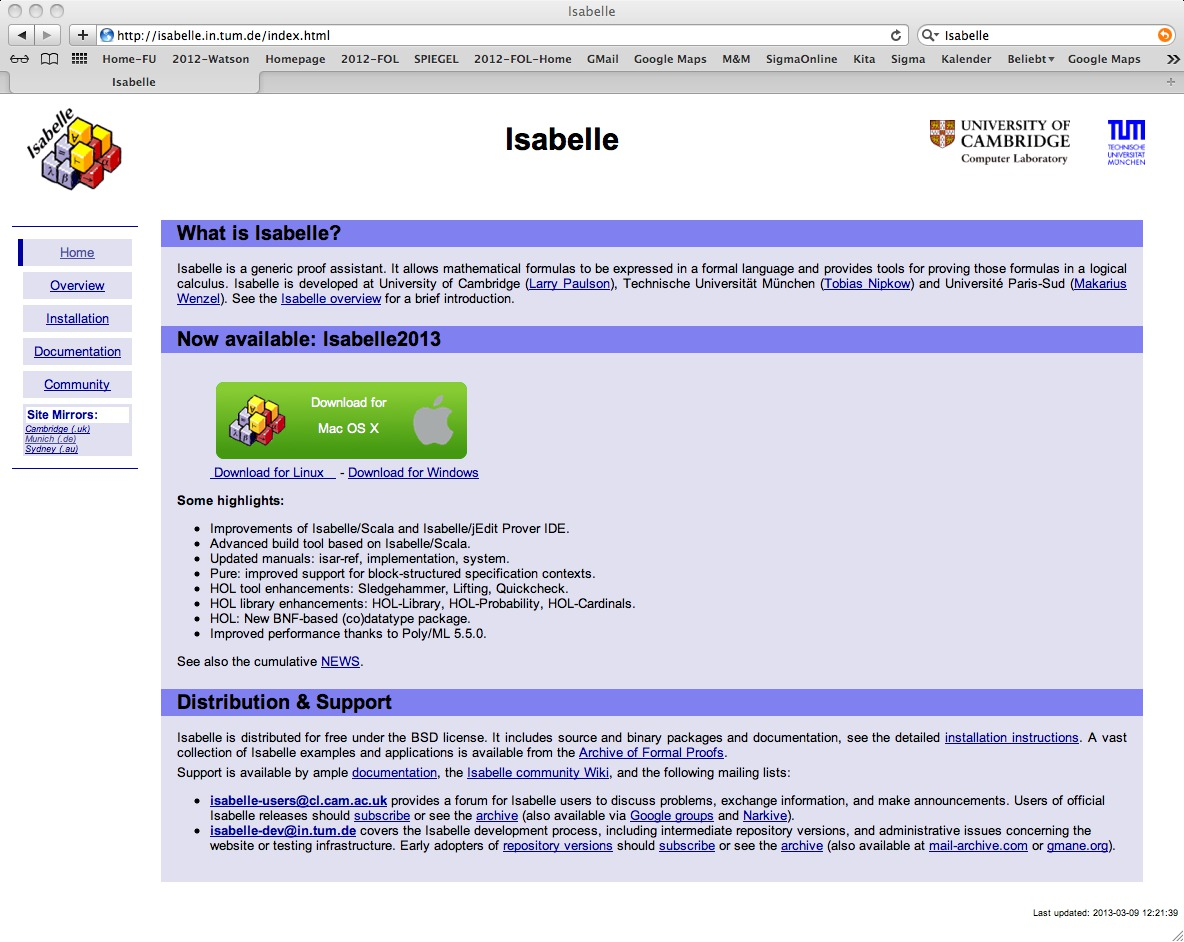
\includegraphics[width=\textwidth]{IsabelleGrab}} 
\end{frame}


\begin{frame}{Automation \& Verification in Proof Assistant \textsc{Isabelle/HOL}} \large
Isabelle/HOL   (Cambridge University/TU Munich)
\begin{itemize}
\item HOL instance of the generic \textsc{Isabelle} proof assistant
\item User interaction and proof automation 
\item Automation is supported by \textsc{Sledgehammer} tool
\item Verification of the proofs in \textsc{Isabelle/HOL}'s small proof kernel
\end{itemize}
\vfill
What we did?
\begin{itemize}
\item Proof automation of G\"odel's proof script (Scott version)
\item \textsc{Sledgehammer} makes calls to remote THF provers in Miami
\item These calls the suggest respective calls to the \textsc{Metis} prover
\item \textsc{Metis} proofs are verified in \textsc{Isabelle/HOL}'s proof kernel
\end{itemize}
\vfill
See the handout (generated from the Isabelle source file).
\end{frame}


\begin{frame}{Automation \& Verification in Proof Assistant
    \textsc{Isabelle/HOL}} \large
\colorbox{gray}{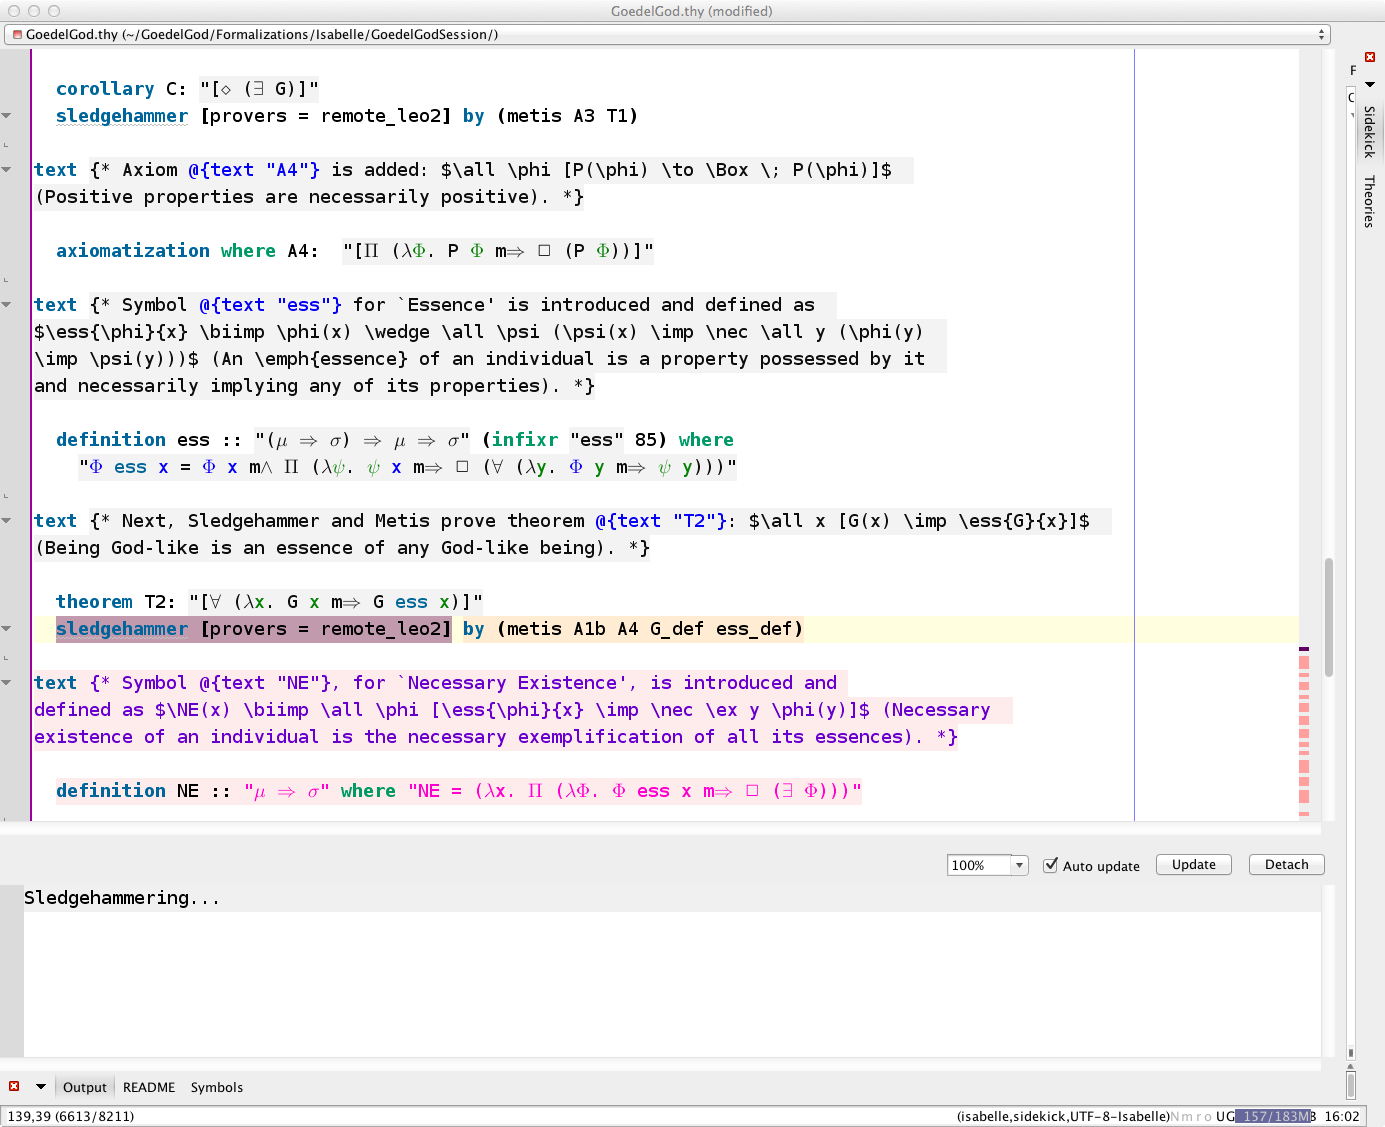
\includegraphics[width=.92\textwidth]{IsabelleDemoGrab}} 
\end{frame}

\begin{transitionframe}{Images/Transitions/NietzscheGod3}{black}
\textbf{Part E:}

Criticisms
\end{transitionframe}

\begin{frame}{Criticisms}{S5} \centering
$$
\all P.[ \pos \nec P \imp \nec P ] 
$$

\medskip

If something is possibly necessary, then it is necessary.

\pause

\bigskip


$
\pos\only<8->{_c} \nec\only<8->{_c} (A \vee \neg A)
$
\pause
\qquad 
$
\nec\only<8->{_c} (A \vee \neg A)
$

\pause

\bigskip

logical necessity $\sim$ validity
%\qquad\qquad
\hfill
logical possibility $\sim$ satisfiability

\pause 

\medskip

$ 
\textrm{for all } M, M \models F 
\quad \longrightarrow \quad
\nec F
%\qquad\qquad\quad
\hfill
\textrm{exists } M, M \models F 
\quad \longrightarrow \quad
\pos F
$

\pause

\bigskip

\textbf{What about iterations?}
$$
\pos \nec \pos \pos F
$$

\medskip

\pause

weak intuitions $\Rightarrow$ dozens of modal logics

\medskip

\pause

\alert{S5 is considered adequate}

\medskip

\pause

\textcolor{blue}{(But KB is sufficient!)}


\end{frame}


\begin{frame}{Criticisms}{Modal Collapse} \centering
$$
\all P.[ P \imp \nec P ] 
$$

\medskip

Everything that is the case is so necessarily.

\pause

\medskip

Follows from T2, T3 and D2.

\pause

\medskip

There are no contingent ``truths''. \\ \pause
Everything is determined. \\ \pause
There is no free will. \\ \pause


\pause
\bigskip

Many proposed solutions: Anderson, Fitting, H\'ajek, \ldots
 
\end{frame}


\begin{frame}{Criticisms}{No Neutral Properties} \centering

$$\all \phi [P(\neg \phi) \biimp \neg P(\phi)]$$

Either a property is positive or its negation is (but never both)
		  
\pause
\bigskip

Are the following properties positive or negative?

$$
\lambda x. G(x) \qquad \lambda x. E(x) \qquad \lambda x. x = x  \qquad  \lambda x. \top
$$
\pause
$$
\lambda x. blue(x) \pause \qquad \lambda x. white(x) \pause \qquad \lambda x. human(x)
$$

%\pause

%$$
%\lambda x. foreigner(x) \qquad \lambda x. \neg foreigner(x), \ldots
%$$

\pause
\bigskip

Solution: \\
``\ldots positive in the moral aesthetic sense (independently of the accidental structure of the world). Only then the ax. true. \ldots''
\\ \hfill - G\"odel, 1970
\end{frame}





\begin{transitionframe}
\textbf{Part F:}

Conclusions
\end{transitionframe}



\begin{frame}{Summary of Results} \large

The (\alert{new}) insights we gained from experiments include:\\[.5em]
\begin{itemize}
\item Logic K sufficient for T1, C and T2 
\item Logic S5 not needed for T3
\item \alert{Logic KB sufficient for T3 (not well known)}
\item \alert{We found a simpler new proof of C}
\item \alert{G\"odel's axioms (without conjunct $\phi(x)$ in D2) are inconsistent}
\item Scott's axioms are consistent
\item For T1, only half of A1 (A1a) is needed 
\item For T2, the other half (A1b) is needed
\end{itemize}
\end{frame}


\begin{frame}{Summary of Results} \large

Our novel contributions the  theorem proving community includes \\[.5em]
\begin{itemize}
\item Powerful infrastructure for reasoning with higher-order modal logic using existing proof assistants and HOL provers
\item A new natural deduction calculus for higher-order modal logic
\item Difficult new benchmarks problems for HOL provers
\item Huge media attention
\end{itemize}
\end{frame}

\begin{frame}{Conclusion} \large
\vskip-1em What have we achieved \\[.5em]
\begin{itemize}
\item Verification of G\"odel's ontological argument with HOL provers
  \begin{itemize}
  \item exact parameters known: constant domain quantification, Henkin Semantics
  \item parameters can be varied and experiments can repeated
  \end{itemize}
\item Gained some novel results and insights
\item Major  step towards \alert{Computer-assisted Theoretical Philosophy}
 \begin{itemize}
  \item see also Ed Zalta's \emph{Computational Metaphysics} project at Stanford University
  \item remember Leibniz' dictum --- \emph{Calculemus!}
  \end{itemize}
\item Interesting bridge between CS, Philosophy and Theology
\end{itemize}

\pause

\vfill
\vskip-1em Ongoing and future work \\[.5em]
\begin{itemize}
\item Formalize and verify literature on ontological arguments
  \begin{itemize}
  \item \ldots in particular the criticism and improvements to G\"odel 
  \end{itemize}
\item Own contributions --- supported by theorem provers
\end{itemize}
\end{frame}


\begin{frame}{Some Comments and Reactions}
\colorbox{gray}{
\includegraphics[width=.8\textwidth]{Comment1}}\\[.7em]

\, \hfill \colorbox{gray}{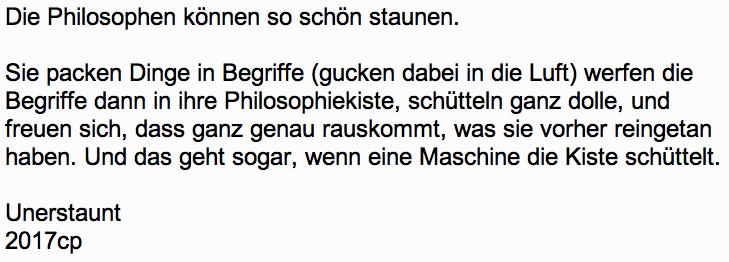
\includegraphics[width=.7\textwidth]{Comment2}}\\[.7em]

\colorbox{gray}{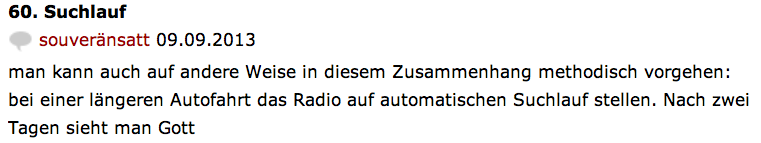
\includegraphics[width=.8\textwidth]{Comment3}}\\[1em]

\, \hfill \ldots find more on the internet \ldots
\end{frame}

\begin{frame}[plain]
\colorbox{black}{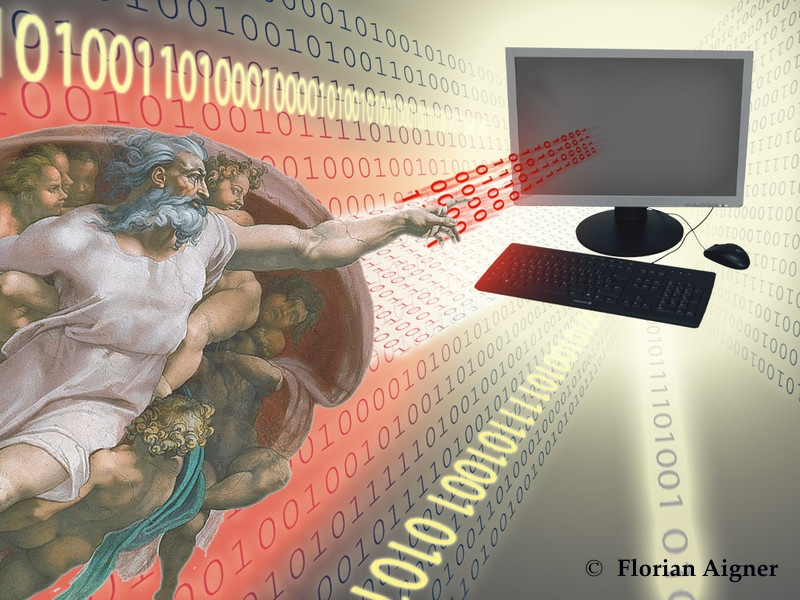
\includegraphics[width=\textwidth]{TUWien-GodComputerC}}
\end{frame}


\end{document}
